\chapter{Additional Figures and Tables}

This appendix collects supporting diagnostics and exploratory analyses that
complement the primary results. Figures based on the final intervention use
$n=983$ eligible episodes and relative edit size $r=0.2$ unless stated
otherwise. Exploratory comparisons are identified explicitly and should not be
interpreted as prespecified primary tests.

\section{Source-Data Integrity}

\begin{figure}[H]
    \centering
    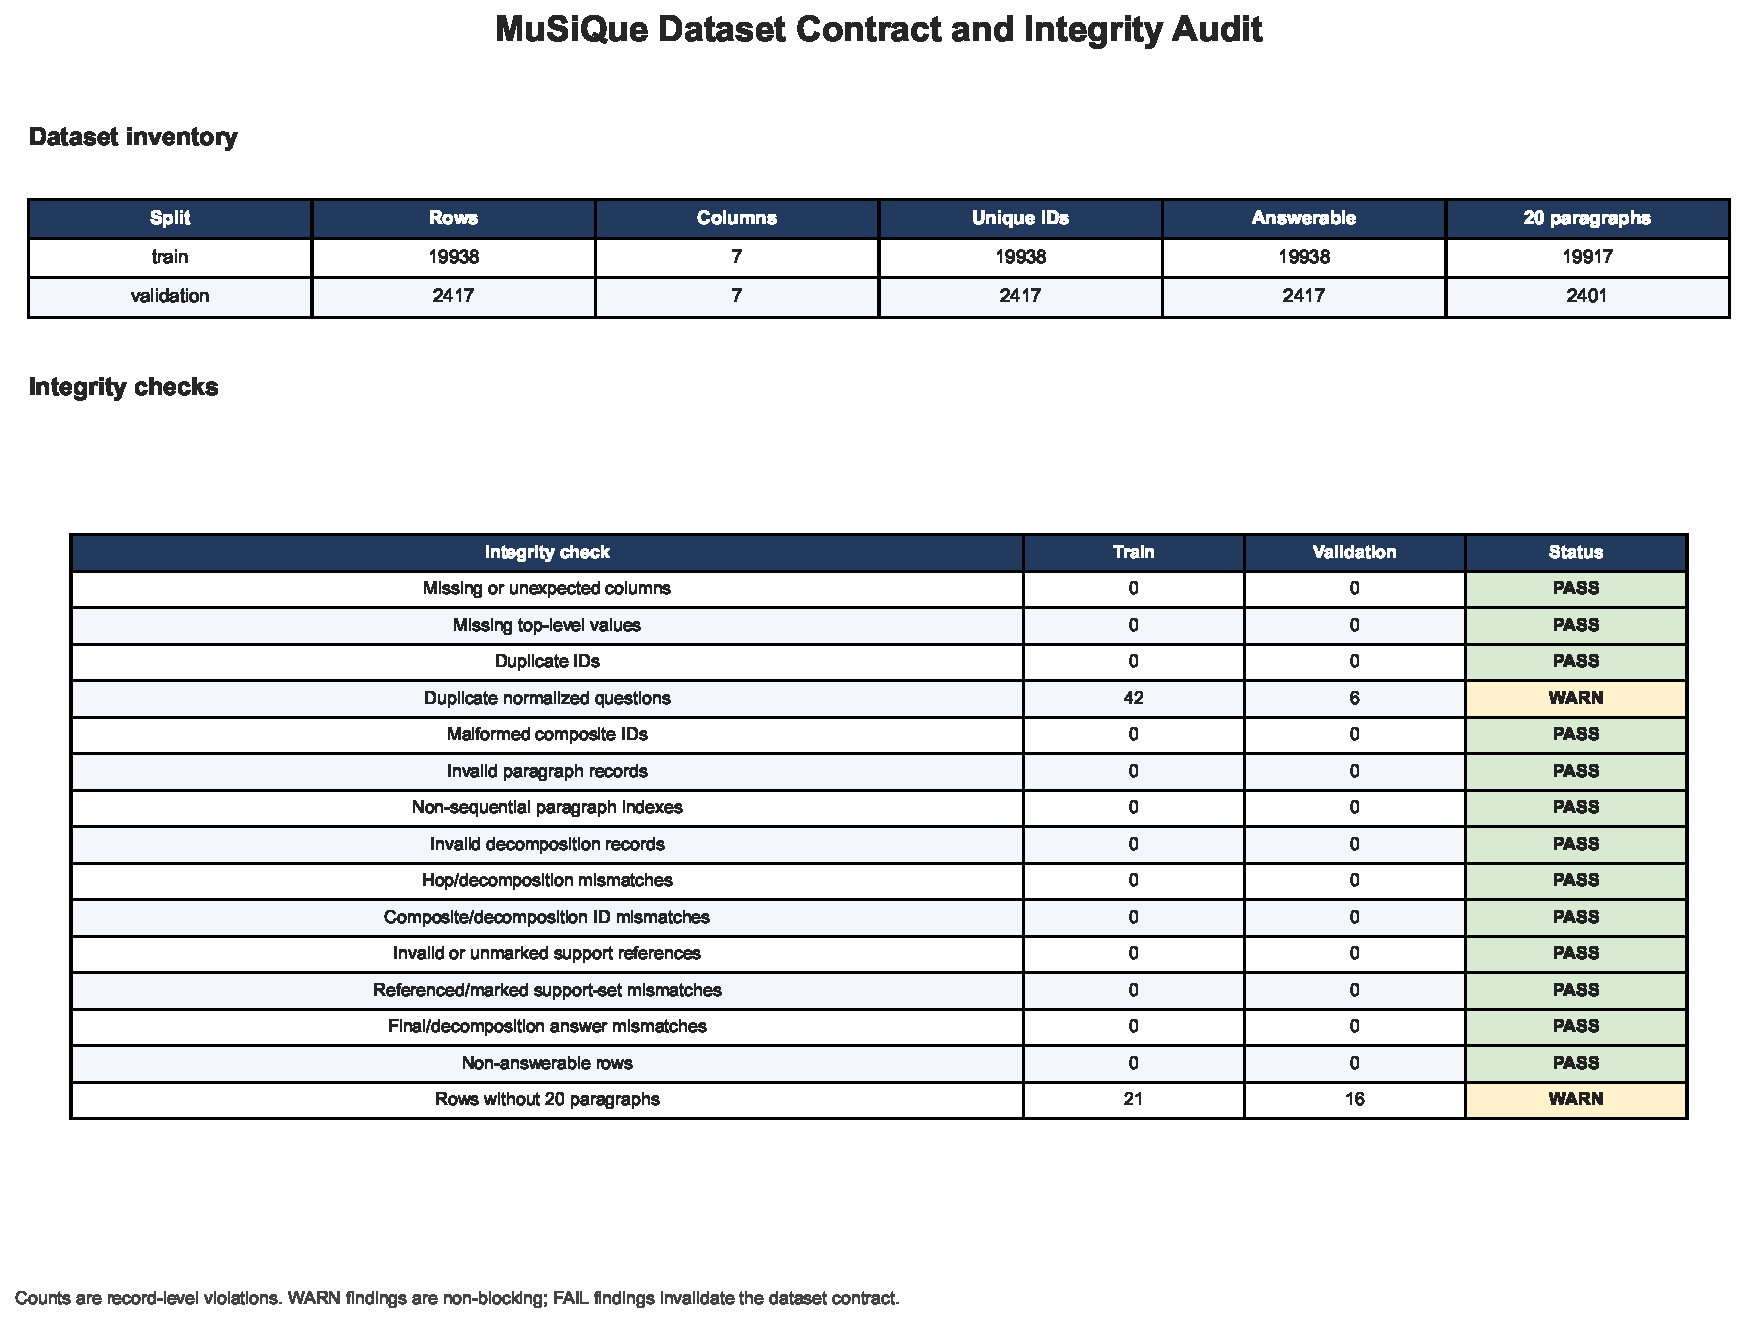
\includegraphics[width=0.95\textwidth,height=0.78\textheight,keepaspectratio]
    {build_figures/dataset_schema_and_integrity_audit.pdf}
    \caption{Contract and integrity audit for the source MuSiQue train and
    validation files. The counts describe the source dataset before the final
    mixed corpus was assembled; warnings are retained as descriptive data
    characteristics rather than silently removed.}
    \label{fig:appendix-dataset-integrity}
\end{figure}

\clearpage
\section{Feature-Selection Diagnostic}

\begin{figure}[H]
    \centering
    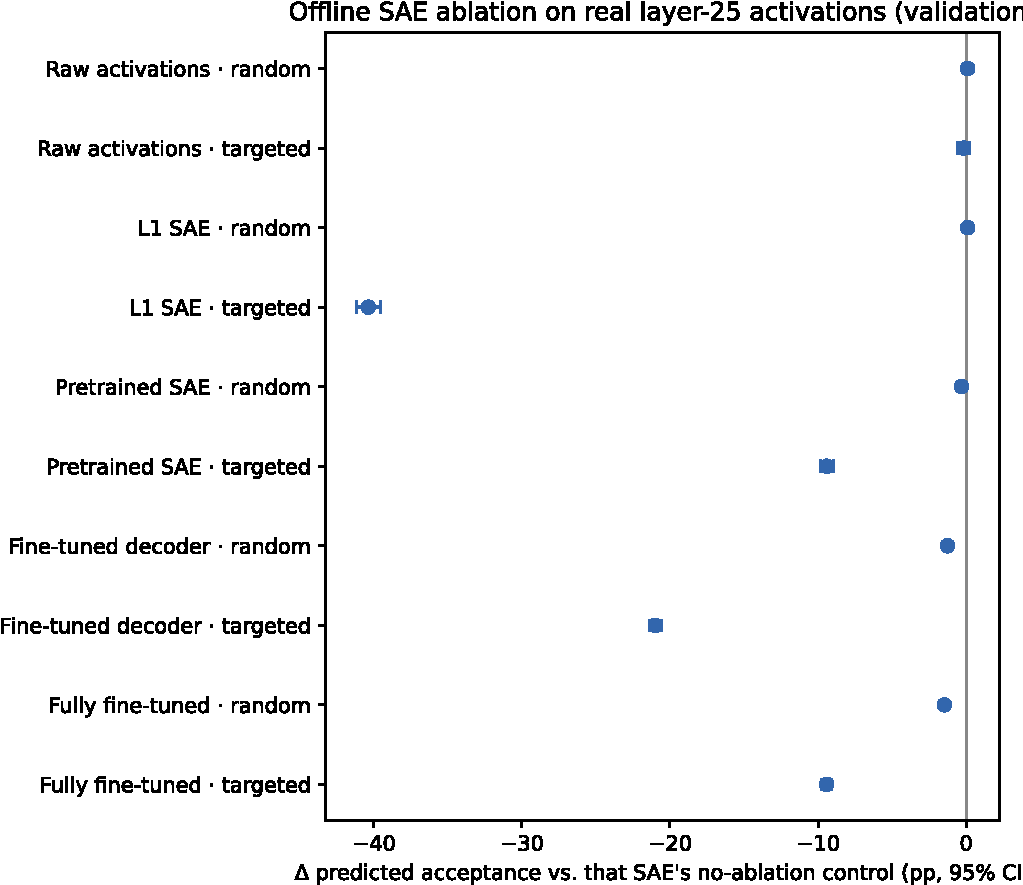
\includegraphics[width=0.92\textwidth,height=0.78\textheight,keepaspectratio]
    {build_figures/feature_selection_causal_proxy_effects.pdf}
    \caption{Offline validation-set ablation diagnostic for the final Layer 25
    feature-selection run. Points report the change in predicted acceptance
    under targeted and random feature ablations, with 95\% confidence
    intervals. This diagnostic supported feature selection but is not an
    autoregressive causal-intervention result.}
    \label{fig:appendix-feature-selection-proxy}
\end{figure}

\clearpage
\section{Causal-Intervention Robustness Checks}

\begin{figure}[H]
    \centering
    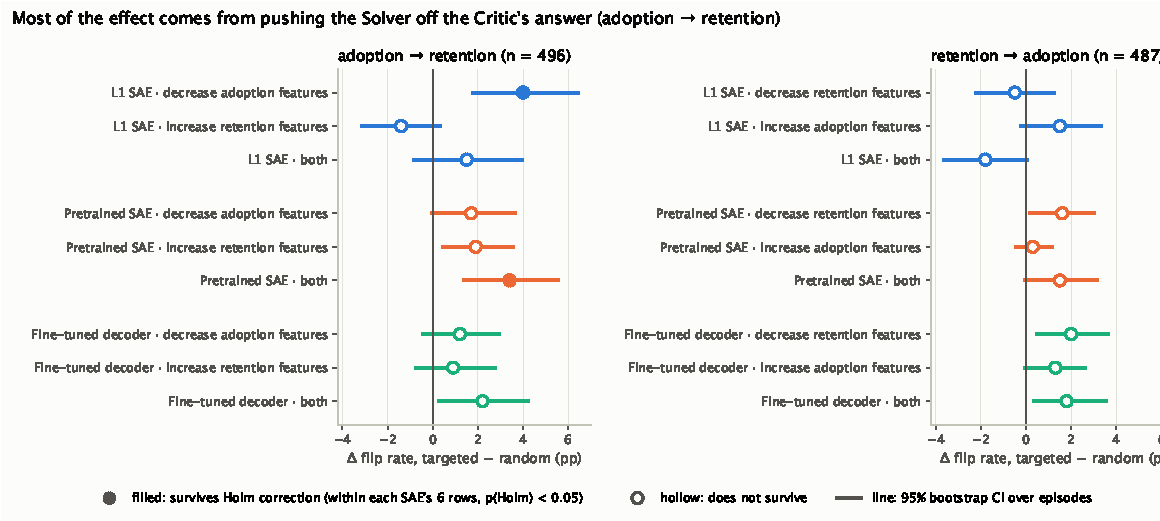
\includegraphics[width=\textwidth,height=0.76\textheight,keepaspectratio]
    {build_figures/intervention_directional_strata.pdf}
    \caption{Targeted-minus-random flip-rate effects separated by the baseline
    decision direction. Filled points show adoption-to-retention episodes and
    hollow points show retention-to-adoption episodes; intervals are 95\%
    bootstrap confidence intervals.}
    \label{fig:appendix-directional-strata}
\end{figure}

\begin{figure}[H]
    \centering
    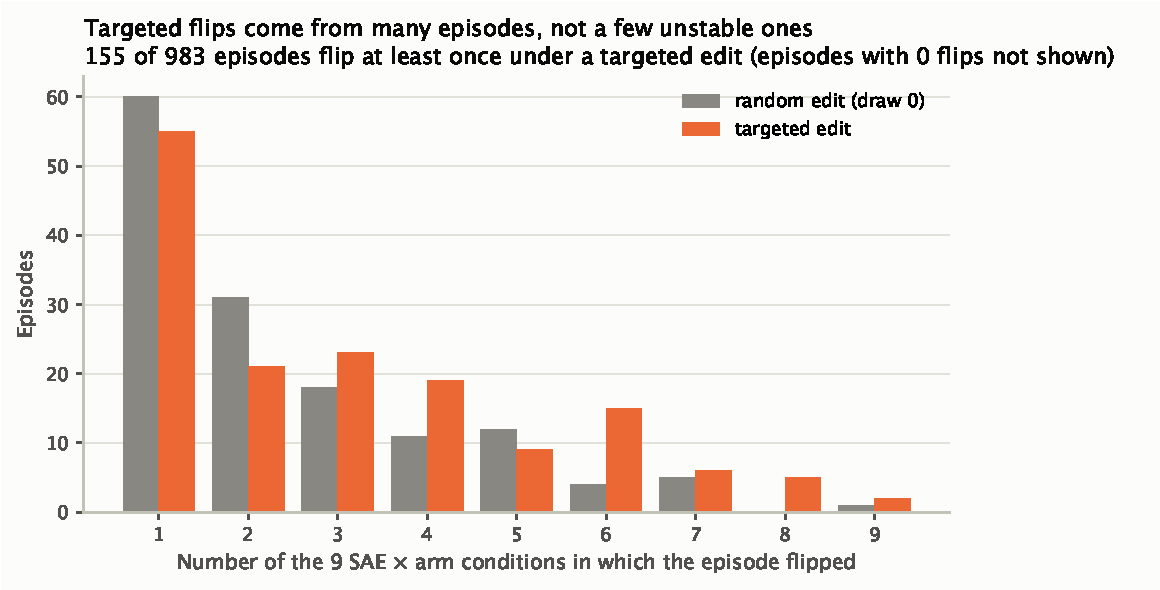
\includegraphics[width=0.95\textwidth,height=0.76\textheight,keepaspectratio]
    {build_figures/intervention_flip_distribution.pdf}
    \caption{Distribution of the number of SAE-by-arm conditions in which an
    episode flipped. Episodes with no flips are omitted from the plotted
    histogram; the comparison checks whether aggregate effects were driven by
    only a few unstable episodes.}
    \label{fig:appendix-flip-distribution}
\end{figure}

\begin{figure}[H]
    \centering
    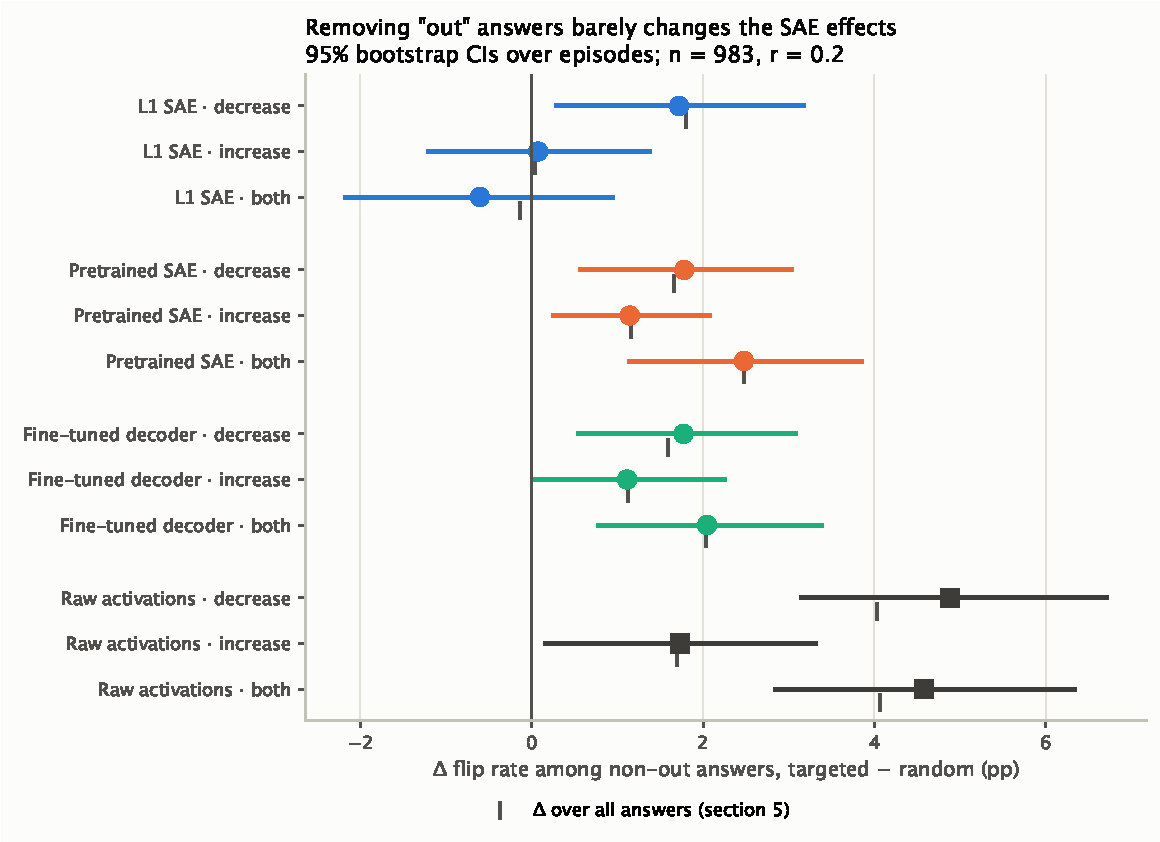
\includegraphics[width=0.86\textwidth,height=0.76\textheight,keepaspectratio]
    {build_figures/intervention_non_out_robustness.pdf}
    \caption{Targeted-minus-random flip-rate effects after restricting the
    analysis to generated answers assigned one of the two candidate labels.
    Black marks reproduce the corresponding all-answer estimates for
    comparison.}
    \label{fig:appendix-non-out-robustness}
\end{figure}

\begin{figure}[H]
    \centering
    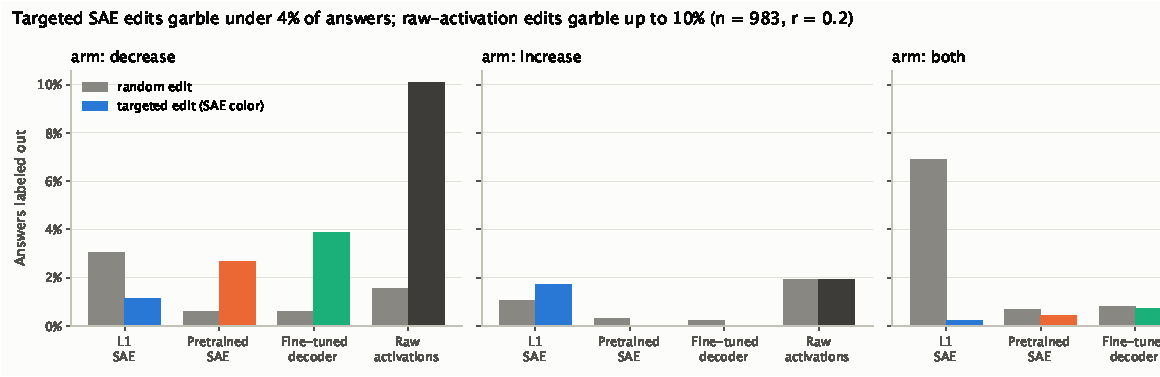
\includegraphics[width=\textwidth,height=0.70\textheight,keepaspectratio]
    {build_figures/intervention_out_rate.pdf}
    \caption{Rate at which targeted and random edits produced answers outside
    the two candidate labels, separated by representation and intervention
    arm. This diagnostic distinguishes behavioral switching from generation
    derailment.}
    \label{fig:appendix-out-rate}
\end{figure}

\begin{figure}[H]
    \centering
    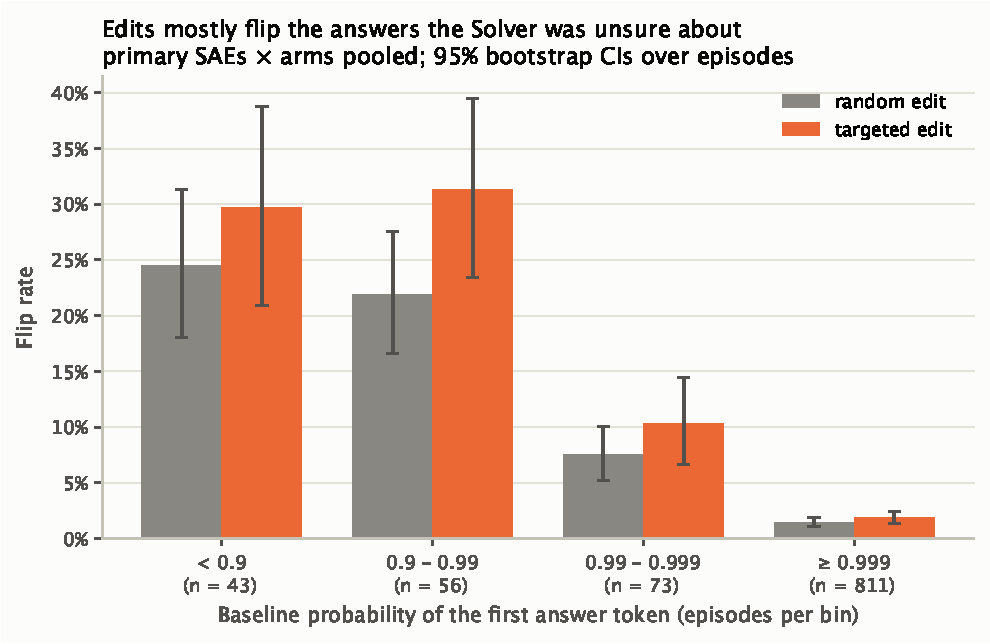
\includegraphics[width=0.92\textwidth,height=0.72\textheight,keepaspectratio]
    {build_figures/intervention_confidence_sensitivity.pdf}
    \caption{Flip rates stratified by the Solver's baseline probability for
    its first answer token. Results pool the primary SAE families and
    intervention arms; error bars are 95\% bootstrap confidence intervals over
    episodes.}
    \label{fig:appendix-confidence-sensitivity}
\end{figure}

\clearpage
\section{Exploratory Adaptation and Editing Checks}

\begin{figure}[H]
    \centering
    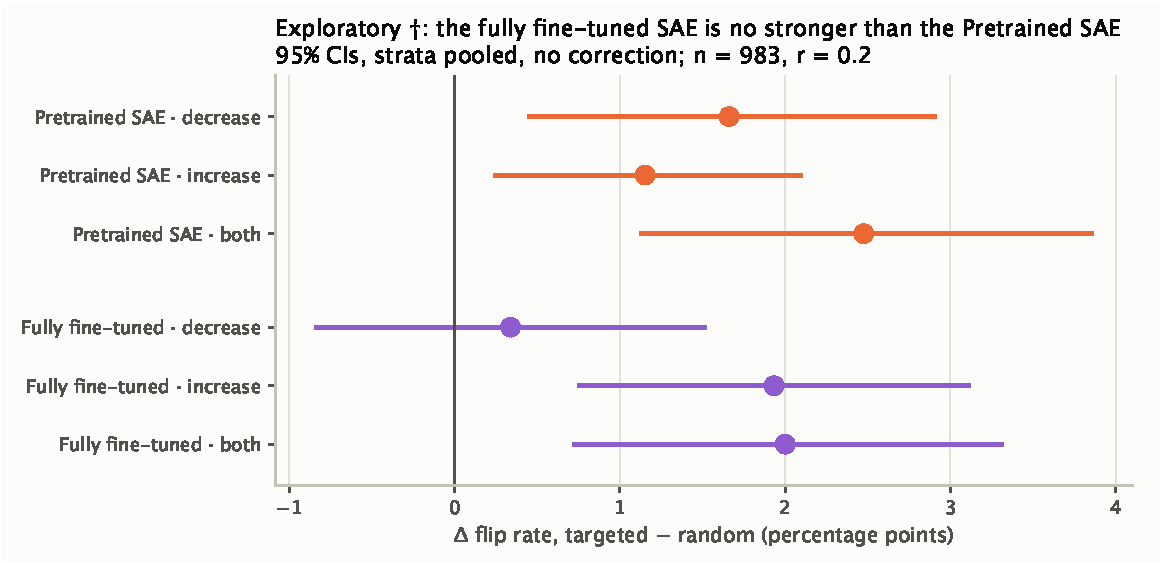
\includegraphics[width=0.94\textwidth,height=0.72\textheight,keepaspectratio]
    {build_figures/intervention_full_finetuning_exploratory.pdf}
    \caption{Exploratory comparison of the fully fine-tuned SAE with the frozen
    pretrained SAE. Effects are targeted-minus-random flip-rate differences
    with uncorrected 95\% confidence intervals; this comparison was not part of
    the prespecified primary family.}
    \label{fig:appendix-full-finetuning}
\end{figure}

\begin{figure}[H]
    \centering
    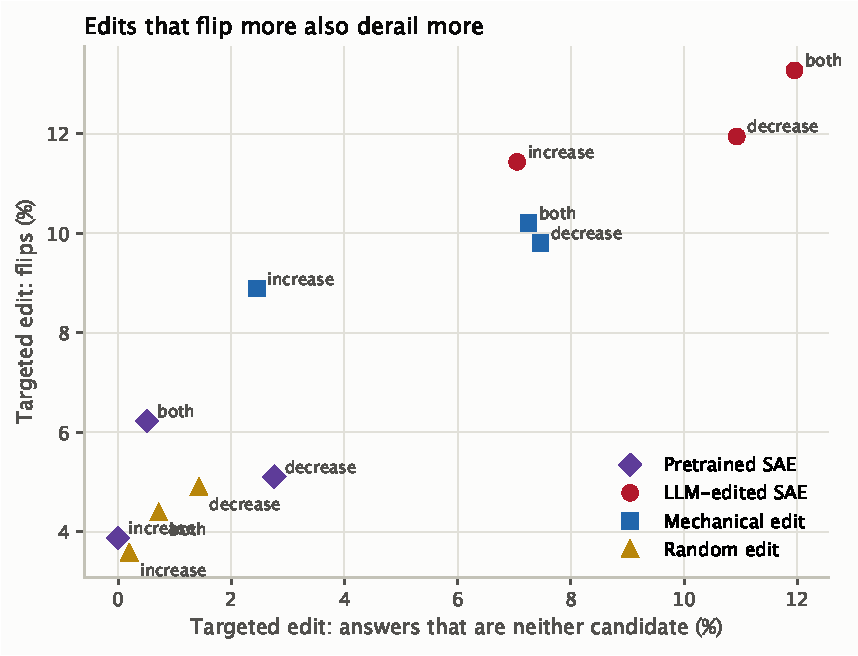
\includegraphics[width=0.84\textwidth,height=0.72\textheight,keepaspectratio]
    {build_figures/llm_edit_flips_vs_out.pdf}
    \caption{Exploratory relationship between targeted flip rates and
    out-of-candidate answer rates for the frozen pretrained, LLM-edited,
    mechanical-control, and random-control SAEs. The plot is diagnostic: a
    higher flip rate is not necessarily desirable when accompanied by more
    out-of-candidate generations.}
    \label{fig:appendix-llm-edit-flips-vs-out}
\end{figure}
